\section{Phần 4 -- Navigation với Nav2}

\subsection{Khởi chạy}
Nav2 chạy \emph{sau} localization (AMCL cung cấp TF \code{map}$\to$\code{odom} và \code{map\_server} cung cấp \code{/map}) và sau khi đã đặt initial pose:
\begin{lstlisting}[language=bash,caption={\file{scripts/start\_nav2.sh}.}]
exec ros2 launch turtlebot4_navigation nav2.launch.py use_sim_time:=true \
  params_file:="$DIR/config/nav2.yaml" "$@"
\end{lstlisting}
Launch này gọi \code{nav2\_bringup/navigation\_launch.py}, đặt lại tên \code{cmd\_vel}: controller phát \code{cmd\_vel\_nav}, \code{velocity\_smoother}
làm mượt rồi phát \code{cmd\_vel} (topic mà \code{motion\_control} của robot nhận). Log xác nhận các node đã \emph{active}:
\begin{lstlisting}[numbers=none,basicstyle=\ttfamily\footnotesize,caption={Cuối log \code{start\_nav2.sh}.}]
[lifecycle_manager_navigation]: Server velocity_smoother connected with bond.
[lifecycle_manager_navigation]: Managed nodes are active
\end{lstlisting}

\subsection{Nav2 lập kế hoạch và điều khiển như thế nào}
\begin{figure}[H]\centering
\small
\begin{tabular}{c}
Goal (RViz2 \emph{Nav2 Goal} $\rightarrow$ action \code{navigate\_to\_pose})\\
$\downarrow$\\
\textbf{bt\_navigator} (cây hành vi: lập kế hoạch lại $+$ phục hồi)\\
$\downarrow$ \code{compute\_path\_to\_pose}\hspace{2cm}$\downarrow$ \code{follow\_path}\\
\textbf{planner\_server} (NavFn) \hspace{1cm}$\rightarrow$ \code{/plan} $\rightarrow$\hspace{1cm} \textbf{controller\_server} (DWB)\\
dùng \textbf{global\_costmap}\hspace{4.2cm}dùng \textbf{local\_costmap}\\
$\downarrow$\\
\code{/cmd\_vel\_nav} $\rightarrow$ \textbf{velocity\_smoother} $\rightarrow$ \code{/cmd\_vel} $\rightarrow$ \code{motion\_control} $\rightarrow$ bánh xe\\
\end{tabular}
\caption{Luồng dữ liệu của Nav2 trong bài.}
\end{figure}

\paragraph{Bản đồ chi phí (costmap).} \code{global\_costmap} (frame \code{map}, cập nhật 1\,Hz) gồm \code{static\_layer} (từ \code{/map}),
\code{obstacle\_layer} (từ \code{/scan}) và \code{inflation\_layer}. \code{local\_costmap} (frame \code{odom}, cửa sổ trượt $3\times 3$\,m, 5\,Hz) dùng
\code{voxel\_layer}. \code{inflation\_layer} làm phồng vật cản: các ô trong bán kính \code{inflation\_radius} quanh tường có chi phí giảm dần
theo $\exp(-\text{cost\_scaling\_factor}\cdot(d-r_{\text{robot}}))$, nên đường đi tránh sát tường.
\begin{lstlisting}[language=yaml,caption={Trích \file{config/nav2.yaml}: costmap.}]
robot_radius: 0.175
inflation_layer:
  plugin: "nav2_costmap_2d::InflationLayer"
  cost_scaling_factor: 4.0
  inflation_radius: 0.45
obstacle_layer / voxel_layer:
  observation_sources: scan
  raytrace_max_range: 3.0
  obstacle_max_range: 2.5
\end{lstlisting}

\paragraph{Lập kế hoạch toàn cục (planner\_server).} Dùng \code{nav2\_navfn\_planner/NavfnPlanner} (Dijkstra, \code{use\_astar: false}) trên \code{global\_costmap};
\code{tolerance: 0.5} cho phép goal lệch tối đa 0,5\,m nếu ô goal không đi được. Kết quả là đường đi ngắn nhất tránh vùng chi phí cao, phát trên \code{/plan}.
\begin{lstlisting}[language=yaml,caption={Trích \file{config/nav2.yaml}: planner.}]
planner_server:
  ros__parameters:
    expected_planner_frequency: 20.0
    planner_plugins: ["GridBased"]
    GridBased:
      plugin: "nav2_navfn_planner/NavfnPlanner"
      tolerance: 0.5
      use_astar: false
\end{lstlisting}

\paragraph{Điều khiển cục bộ (controller\_server).} Chạy ở 20\,Hz với \code{dwb\_core::DWBLocalPlanner} (Dynamic Window Approach). Mỗi chu kỳ DWB lấy mẫu
các cặp $(v,\omega)$ khả dĩ trong cửa sổ động (giới hạn tốc độ và gia tốc), mô phỏng quỹ đạo \code{sim\_time}=1,7\,s về phía trước trên \code{local\_costmap},
chấm điểm từng quỹ đạo bằng các \emph{critic} và chọn quỹ đạo điểm tốt nhất: \code{BaseObstacle} (tránh vật cản), \code{PathAlign}/\code{PathDist}
(bám đường toàn cục), \code{GoalAlign}/\code{GoalDist} (tiến gần goal), \code{RotateToGoal} (xoay đúng hướng ở đích), \code{Oscillation} (chống dao động).
\begin{lstlisting}[language=yaml,caption={Trích \file{config/nav2.yaml}: controller.}]
controller_server:
  ros__parameters:
    controller_frequency: 20.0
    general_goal_checker:
      plugin: "nav2_controller::SimpleGoalChecker"
      xy_goal_tolerance: 0.25
      yaw_goal_tolerance: 0.25
    FollowPath:
      plugin: "dwb_core::DWBLocalPlanner"
      max_vel_x: 0.26      max_vel_theta: 1.0
      acc_lim_x: 2.5       acc_lim_theta: 3.2
      vx_samples: 20       sim_time: 1.7
      critics: ["RotateToGoal", "Oscillation", "BaseObstacle", "GoalAlign",
                "PathAlign", "PathDist", "GoalDist"]
\end{lstlisting}

\paragraph{Cây hành vi và phục hồi (bt\_navigator, behavior\_server).} Mặc định dùng cây
\code{navigate\_to\_pose\_w\_\allowbreak replanning\_and\_\allowbreak recovery}: lập kế hoạch lại định kỳ, theo đường đi; nếu thất bại thì xóa costmap và chạy các hành vi phục hồi
của \code{behavior\_server} (\code{spin}, \code{backup}, \code{wait}, ...) rồi thử lại. Goal chỉ ``thành công'' khi robot vào trong
\code{xy\_goal\_tolerance}=0,25\,m (và đúng hướng trong 0,25\,rad).

\paragraph{Làm mượt vận tốc.} \code{velocity\_smoother} giới hạn tốc độ $\pm0{,}26$\,m/s, $\pm1{,}0$\,rad/s và gia tốc $2{,}5$\,m/s$^2$, $3{,}2$\,rad/s$^2$ trước khi gửi \code{/cmd\_vel}.

\subsection{Thực hiện navigation goal}
Sau khi AMCL đã hội tụ (Phần 3), em đặt goal. Trong video demo, goal được đặt bằng công cụ \emph{Nav2 Goal} của RViz2 (không lái tay sau đó).
Để có số liệu có thể kiểm chứng (thời gian, quãng đường, khoảng cách tối thiểu tới tường), em còn dùng \file{scripts/send\_goals.py}, gửi cùng loại goal
\code{NavigateToPose} qua action server và ghi lại vị trí AMCL và khoảng cách nhỏ nhất của \code{/scan}:
\begin{lstlisting}[language=Python,caption={Trích \file{scripts/send\_goals.py}.}]
client = ActionClient(node, NavigateToPose, 'navigate_to_pose')
msg = NavigateToPose.Goal()
msg.pose.header.frame_id = 'map'
msg.pose.pose.position.x, msg.pose.pose.position.y = gx, gy
msg.pose.pose.orientation.z, msg.pose.pose.orientation.w = math.sin(gyaw/2), math.cos(gyaw/2)
fut = client.send_goal_async(msg)
\end{lstlisting}
Bốn goal ở bốn khu vực khác nhau của bản đồ (tọa độ trong frame \code{map}):
\begin{table}[H]\centering\small
\begin{tabular}{clcccc}\toprule
Goal & Khu vực & Tọa độ & Kết quả & Quãng đường & Cách tường gần nhất\\\midrule
1 & phải-giữa, gần hộp & (3,0; 2,0) & thành công (lần 2) & 1,62\,m & 0,37\,m\\
2 & hành lang phía bắc & (2,5; 5,6) & thành công & 7,41\,m & 0,46\,m\\
3 & góc tây-bắc, cạnh hộp & ($-0{,}4$; 5,6) & thành công & 2,60\,m & 0,48\,m\\
4 & đông-nam & (3,5; 0,2) & thành công & 6,73\,m & 0,41\,m\\
\bottomrule\end{tabular}
\caption{Kết quả bốn goal (nguồn: \file{logs/04\_nav\_goals.log}, \file{logs/05\_nav\_goal1\_retry.log}). Sai số tới đích đo bằng \code{/amcl\_pose} sau khi goal kết thúc: 0,21; 0,20; 0,28; 0,19\,m (goal 1--4). Goal checker xác nhận ``thành công'' với ngưỡng 0,25\,m; số 0,28\,m của goal 3 hơi lớn hơn ngưỡng. Em chưa xác định chắc lý do; có thể do \code{/amcl\_pose} chỉ cập nhật khi robot đi đủ \code{update\_min\_d}=0,25\,m nên giá trị em đọc có thể cũ, hoặc do sai số định vị AMCL, nên không nên coi con số này chính xác hơn vài cm.}\label{tab:goals}
\end{table}
\paragraph{Về goal 1.} Lần đầu goal 1 bị \emph{ABORTED}: planner báo
\emph{``Planning algorithm GridBased failed to generate a valid path to (3.00, 2.00)''}, robot chỉ đi 0,85\,m.
Đến khi chạy lại goal này (sau goal 2--4) thì thành công trong 39\,s. Em chưa xác định chắc nguyên nhân thất bại lần đầu; thời điểm đó
AMCL vừa hội tụ và robot ở gần vị trí xuất phát, nên có thể do costmap/định vị chưa ổn định hoặc robot đứng trong vùng phồng của vách. Vì thế 3 goal liên tiếp đầu tiên
đạt yêu cầu là goal 2, 3, 4; goal 1 thành công ở lần thử lại.

\paragraph{Va chạm.} Khoảng cách nhỏ nhất từ LiDAR tới vật cản trong cả hành trình là 0,37--0,48\,m (robot bán kính 0,175\,m), tức không sát hay chạm tường.
Số liệu này lấy từ \code{/scan} nên chỉ phản ánh vật cản trong mặt phẳng LiDAR. Log của \code{motion\_control} chỉ có các dòng bật reflex lúc khởi động
(\emph{Enabling REFLEX\_BUMP/CLIFF/STUCK/WHEEL\_DROP}), không có sự kiện hazard hay reflex nào trong lúc chạy Nav2; em không ghi riêng topic \code{/hazard\_detection}. Quỹ đạo thật vẽ ở hình dưới.
\begin{figure}[tbp]\centering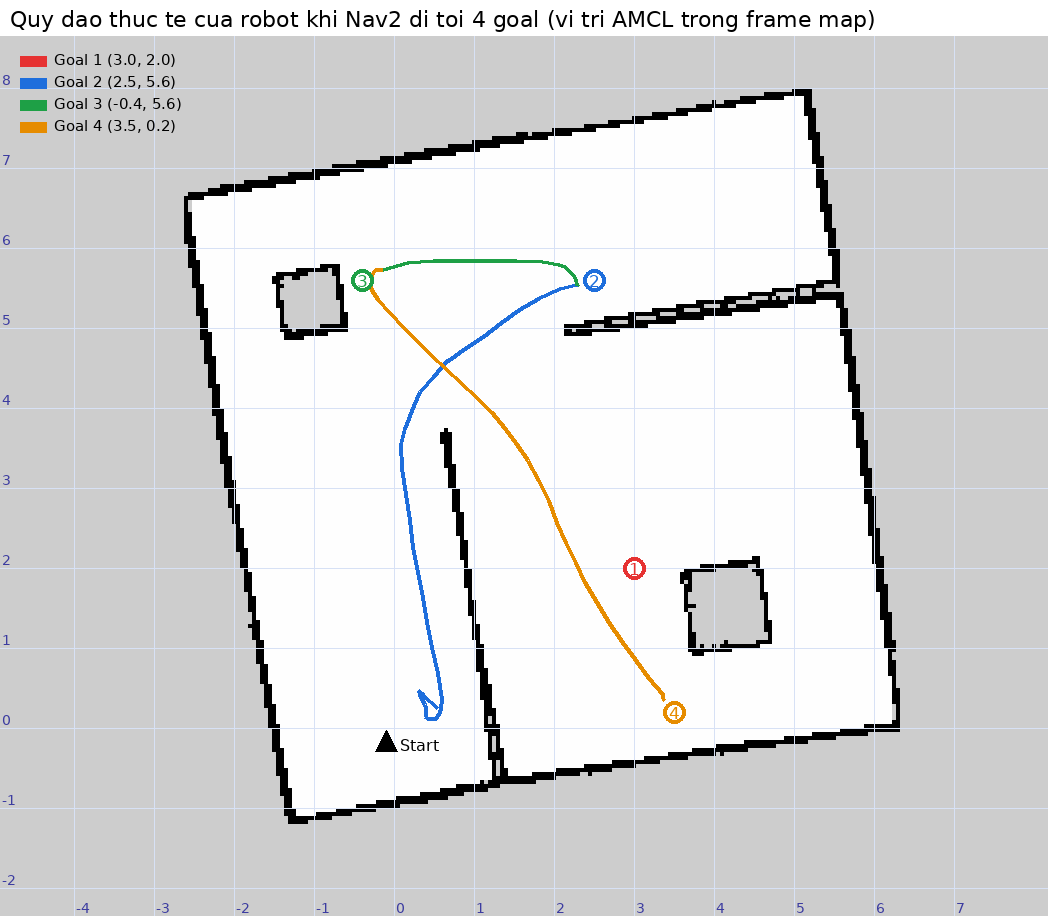
\includegraphics[width=0.9\linewidth]{fig_nav_trajectory.png}
\caption{Quỹ đạo robot (vị trí AMCL) khi Nav2 đi đến goal 2, 3, 4, vẽ trên bản đồ từ \file{logs/nav\_trajectory\_run1.csv}. Số trong vòng tròn là vị trí goal, tam giác đen là vị trí xuất phát. Quỹ đạo của lần chạy lại goal 1 không vẽ được vì file CSV của lần đó đã bị lần gửi goal thứ 5 ghi đè (script lúc đó luôn ghi cùng tên file); chỉ còn số liệu tổng hợp trong \file{logs/05\_nav\_goal1\_retry.log}.}\end{figure}
\begin{figure}[tbp]\centering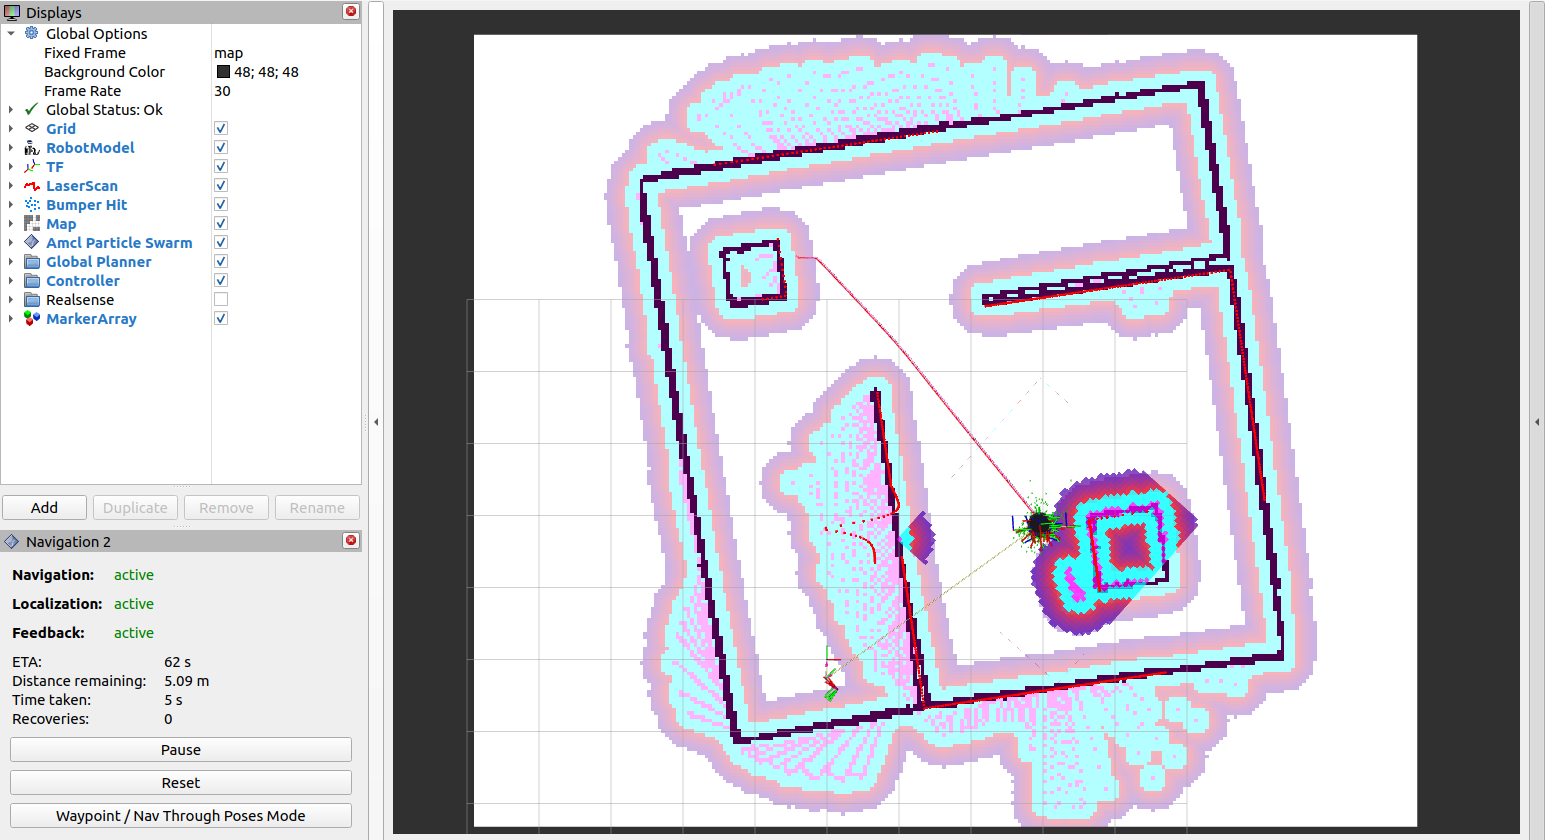
\includegraphics[width=\linewidth]{fig_nav_goal.png}
\caption{RViz2 khi Nav2 đang thực hiện một goal: global costmap (vùng màu quanh tường là inflation), local costmap (ô vuông quanh robot), đường đi toàn cục màu đỏ từ robot tới goal ở góc tây-bắc, hạt AMCL màu xanh lá; bảng \emph{Navigation 2} bên trái báo Navigation/Localization: active. Ảnh chụp ở lần gửi goal thứ 5 (xem mục \ref{sec:goal5}).}\label{fig:navgoal}\end{figure}

\paragraph{Lần gửi goal thứ 5 (thất bại).}\label{sec:goal5} Để chụp Hình~\ref{fig:navgoal}, sau khi hệ thống đã chạy liên tục hơn 2\,200\,s giờ mô phỏng, em gửi lại goal $(-0{,}4;\,5{,}6)$. Planner vẫn tạo được đường đi (Hình~\ref{fig:navgoal}) nhưng robot không tiến được: \code{controller\_server} liên tục báo \emph{``Transform data too old when converting from map to odom''} (TF \code{map}$\to$\code{odom} mà nó giữ có mốc thời gian 1\,235\,s trong khi dữ liệu là 2\,247\,s), rồi \emph{``Failed to make progress''}; hành vi phục hồi \code{spin} cũng thất bại vì \emph{``Current footprint not available''}. Script hủy goal sau 600\,s; robot chỉ dao động quanh chỗ cũ (quãng đường tích lũy 10,4\,m nhưng vị trí thay đổi dưới 0,25\,m) và không va chạm (cách tường $\ge 0{,}50$\,m). Em chưa xác định được nguyên nhân gốc; nghi là bộ đệm TF của Nav2 bị lệch sau một lần RViz2 bị tắt và mở lại, kết hợp máy quá tải (load average 48--60). Vì vậy số liệu chính thức của Phần~4 là 4 goal ở Bảng~\ref{tab:goals}; lần thứ 5 được ghi lại để trung thực (\file{logs/07\_nav\_goal\_rviz\_shot.log}).
